\documentclass[10pt,xcolor=pdflatex,hyperref={unicode}]{beamer}
\usepackage{newcent}
\usepackage[utf8]{inputenc}
\usepackage[czech]{babel}
\usepackage[T1]{fontenc}
\usepackage{hyperref}
\usepackage{booktabs} 
\usetheme{FIT}
\usepackage[newfloat]{minted}
\usepackage{xcolor}
\usepackage{caption}


\definecolor{keyword}{RGB}{167,29,93}
\definecolor{keyword2}{RGB}{56,146,170}
\definecolor{keyword3}{RGB}{116,0,252}

%%%%%%%%%%%%%%%%%%%%%%%%%%%%%%%%%%%%%%%%%%%%%%%%%%%%%%%%%%%%%%%%%%
\title[Typografie a publikování]{Viazaný zoznam}

\author[]{Tomáš Juhász}

\institute[]{Brno University of Technology, Faculty of Information Technology\\
Bo\v{z}et\v{e}chova 1/2. 612 66 Brno - Kr\'alovo Pole\\
\href{mailto:me@somewhere.com}{xjuhas04@fit.vutbr.cz}}

\date{\today}

%%%%%%%%%%%%%%%%%%%%%%%%%%%%%%%%%%%%%%%%%%%%%%%%%%%%%%%%%%%%%%%%%%
\newenvironment{code}{\captionsetup{type=listing}}{}
\SetupFloatingEnvironment{listing}{name= Kód}
\begin{document}

\begin{frame}
\titlepage
\end{frame}
%%%%%%%%%%%%%%%%%%%%%%%%%%
\begin{frame}{Přehled}
	\setbeamertemplate{section in toc}[sections numbered]
	\tableofcontents[hideallsubsections]
\end{frame}
%%%%%%%%%%%%%%%%%%%%%%%%%%
\section {Definicia}
\begin{frame}{Viazaný zoznam}
	\begin{itemize}
		\item
			{\color{keyword}Viazaný zoznam} alebo  linked list alebo viazaný zoznam je dynamická dátová štruktúra 
        \item 
            Skladá sa z prvkov ktoré obsahujú {\color{keyword2}odkaz} na nasledujúci prvok
        \item 
            Základne vlastnosti viazaného zoznamu 			\begin{itemize}
				\item Viazaný zoznam obsahuje odkaz na prvý prvok 
				\item Každý prvok obsahuje dáta a odkaz na nasledujúci prvok 
				\item Posledný prvok obsahuje odkaz na {\color{keyword2}NULL} pre označenie konca zoznamu 
			\end{itemize}
	\end{itemize}
\end{frame}
%%%%%%%%%%%%%%%%%%%%%%%%%%
\begin{frame}{Výhody/Nevýhody}
\begin{itemize}
    \item {\color{keyword}Výhody} 
    \begin{itemize}
        \item Jednoduché vkladanie/mazanie pre dynamicky počet prvkov. 
        \item Efektívne využitie pamäte (alokuje sa iba potrebná pamäť). 
    \end{itemize}
    \item {\color{keyword}Nevýhody}
    \begin{itemize}
        \item K prvkom sa môže pristupovať iba sekvenčne
        \item Vyhľadanie prvkov je  komplexnejšie než pri poli
    \end{itemize}
\end{itemize}
\end{frame}

%%%%%%%%%%%%%%%%%%%%%%%%%%
\begin{frame}[fragile]{Druhy viazaných zoznamov}
	\begin{figure}[h]
		\scalebox{0.55}{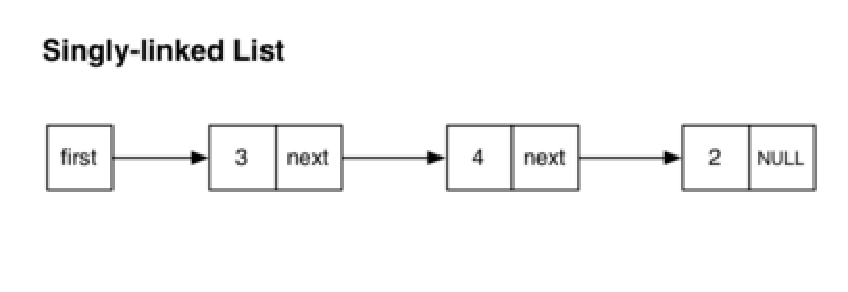
\includegraphics{singlelList.eps}}
		\caption{Obsahuje len ukazovateľa na nasledujúci prvok}
	\end{figure}
	\begin{figure}[h]
		\centering
		\scalebox{0.5}{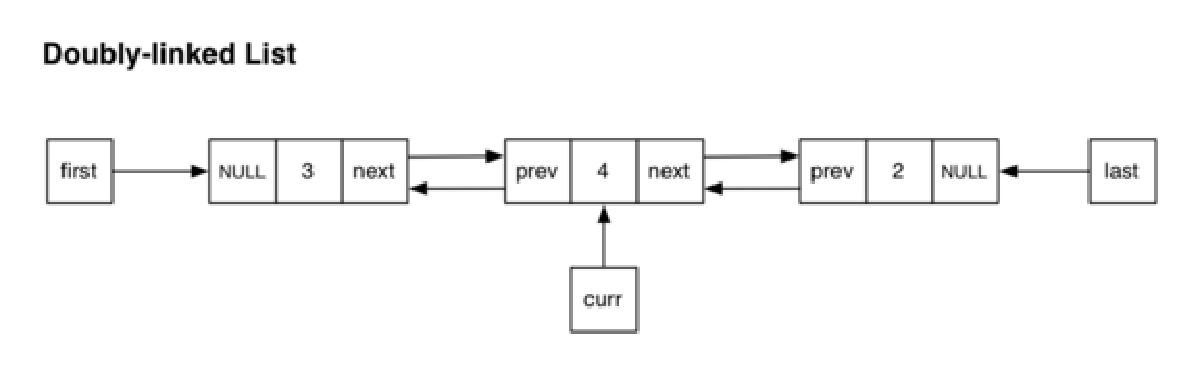
\includegraphics{doublelL.eps}}
		\caption{Obsahuje ukazovateľa aj na predchádzajúci prvok }
	\end{figure}
\end{frame}

%%%%%%%%%%%%%%%%%%%%%%%%%%
\begin{frame}{Časová zložitosť}
\centering
	{\color{keyword}Časová zložitosť} základných operácii  \\

\begin{center}

    \begin{tabular}[center]{ll}
		\toprule
		Operácia  & Zložitosť \\
		\midrule
		Prístup & o(n)\\
		Vyhľadávanie & o(n)\\
		Vkladanie na začiatok & o(1)\\
		Odstránenie zo začiatku & o(1)\\
		Vkladanie na index & o(n)\\
		Odstránenie na indexe & o(n)\\
		\bottomrule
	\end{tabular}
\end{center}
\centering
\begin{itemize}
    \item Pokiaľ sa k prvku potrebujeme dostáť hľadaním je o(n).
    \item Ak stačí prvok iba pridať/odstrániť  na začiatok listu je o (1). 
\end{itemize}
\end {frame}
\section {Operácie}
%%%%%%%%%%%%%%%%%%%%%%%%%%
\begin{frame}{Základne operácie}
    \Large
    \begin{itemize}
        \item
			Základne {\color{keyword}operácie} so zoznamom:
			\begin{enumerate}
			\large
	            \item Inicializácia zoznamu 
				\item Vloženie prvku 
				\item Vymazanie prvku 
				\item Vymazanie zoznamu 
			    \item Prechod zoznamom 
			\end{enumerate}
    \end{itemize}

\end{frame}
\section {Časová zložitosť}
%%%%%%%%%%%%%%%%%%%%%%%%%%
\section {Ukážka kódu}
\begin{frame}[fragile]{Kód štruktúry}
\begin{itemize}
    \item Kód {\color{keyword}štruktúry} môže vyzerať napríklad takto:
\end{itemize}

\centering{
	\begin{minted}[
        frame=lines,
        framesep=2mm,
        baselinestretch=1.2,
        linenos
        ]{c}
	struct listItem{
	    int data;
	    lItem * next
	}
	struct linkedList {
	    lItem * head
	    lItem * tail
	}
	\end{minted}
	}
\captionof{listing}{Samotný {\color{keyword3}list} obsahuje odkaz na {\color{keyword3}prvý} a {\color{keyword3}posledný} prvok}
\end{frame}

\begin{frame}[fragile]{Vloženie prvku}
\begin{itemize}
    \item Pridanie nového prvku na {\color{keyword}začiatok} zoznamu:
\end{itemize}
\begin{minted}[
        frame=lines,
        framesep=2mm,
        baselinestretch=1.2,
        linenos
        ]{c}
    void insertFirst(lList * listItem1)
    {
        lItem * Item2
        newItem2->data = person
        newItem2->next = list->head
        listItem->head    = newItem2
    }
\end{minted}
\captionof{listing}{{\color{keyword3}{Item2}} odkazuje na začiatok zoznamu a {\color{keyword3}{Item1}} na \color{keyword3}{Item2}}
\end{frame}

%%%%%%%%%%%%%%%%%%%%%%%%%%
\begin {frame}[fragile]{Vyhladanie prvku}
\begin{itemize}
    \item {\color{keyword}Vyhladanie} prvku v zozname: 
\end{itemize}
    \begin{minted}[
        frame=lines,
        framesep=2mm,
        baselinestretch=1.2,
        linenos
        ]{c}
    lItem * findItem (lList * list, ldata d)
    {
        lItem * tmp = list->head
        while (tmp != NULL && !isEqual(tmp->data,d)) {
            tmp = list->next
        }
        return tmp
    }
    \end{minted}
    \captionof{listing}{{\color{keyword3}Loop} prejde celý zoznam pokým nenájde {\color{keyword3}dáta} hľadaného prvku}
\end{frame}
%%%%%%%%%%%%%%%%%%%%%%%%%%
\begin{frame}
\frametitle{Použitá literatúra}
\begin{thebibliography}{10}
		\bibitem[Know thy Complexities]{timeComp} Know thy Complexities
		\newblock \texttt{https://www.bigocheatsheet.com/}

		\bibitem[Geeks for Geeks]{gfg} Geeks for Geeks
		\newblock \texttt{https://www.geeksforgeeks.org/linked-list/}

		\bibitem[IZP Dynamicke struktury]{izp} IZP Dynamicke struktury
		\newblock \texttt{https://wis.fit.vutbr.cz/FIT/st/cfs.php/course}
	\end{thebibliography}
\end{frame}

\end{document}
